\documentclass[14pt,a4paper]{extarticle}

\usepackage[utf8]{inputenc}
\usepackage[T2A]{fontenc}
\usepackage{amssymb,amsmath,mathrsfs,amsthm}
\usepackage[russian]{babel}
\usepackage{graphicx}
\usepackage[footnotesize]{caption2}
\usepackage{indentfirst}
\usepackage{multicol}
\usepackage{listings}
\usepackage{float}
\usepackage{url}
\usepackage{hyperref}
\usepackage{enumitem}

%\usepackage[ruled,section]{algorithm}
%\usepackage[noend]{algorithmic}
%\usepackage[all]{xy}
\usepackage{booktabs}
\usepackage{graphicx}
\usepackage[table,xcdraw]{xcolor}
\usepackage{tcolorbox}

%Библиотека для блок-схем
\usepackage{tikz}
\usetikzlibrary{shapes,arrows}

% Параметры страницы
\textheight=24cm
\textwidth=16cm
\oddsidemargin=5mm
\evensidemargin=-5mm
\marginparwidth=36pt
\topmargin=-1cm
\footnotesep=3ex
%\flushbottom
\raggedbottom
\tolerance 3000
% подавить эффект "висячих стpок"
\clubpenalty=10000
\widowpenalty=10000
%\renewcommand{\baselinestretch}{1.1}
\renewcommand{\baselinestretch}{1.5} %для печати с большим интервалом

\newcommand{\angstrom}{\mbox{\normalfont\AA}}

\newtheorem{definition}{Определение} % задаём выводимое слово (для определений)
\newtheorem{example}{Замечание} % задаём выводимое слово (для определений)
\newtheorem{theorem}{Теорема} % задаём выводимое слово (для определений)
\newtheorem{construction}{Конструкция} % задаём выводимое слово (для определений)

\DeclareMathOperator*{\sgn}{sgn}
\DeclareMathOperator*{\var}{var}
\DeclareMathOperator*{\cov}{cov}
\DeclareMathOperator*{\law}{Law}

\newcommand{\1}{\mathbbm{1}}
\newcommand{\R}{\mathbb{R}}
\newcommand{\N}{\mathbb{N}}
\newcommand{\Z}{\mathbb{Z}}
\renewcommand{\P}{\mathbb{P}}
\newcommand{\E}{\mathbb{E}}

\newcommand{\independent}{\perp\!\!\!\!\perp}

\newcommand\cA{{\cal A}}
\newcommand\cE{{\cal E}}
\newcommand\cC{{\cal C}}
\newcommand\cF{{\cal F}}
\newcommand\cG{{\cal G}}
\newcommand\cK{{\cal K}}
\newcommand\cL{{\cal L}}
\newcommand\cB{{\cal B}}
\newcommand\cN{{\cal N}}
\newcommand\cM{{\cal M}}
\newcommand\cX{{\cal X}}
\newcommand\cD{{\cal D}}
\newcommand\cR{{\cal R}}
\newcommand\cP{{\cal P}}
\newcommand\cQ{{\cal Q}}
\newcommand\cS{{\cal S}}
\newcommand\cT{{\cal T}}
\newcommand\cV{{\cal V}}
\newcommand\cZ{{\cal Z}}

\newcommand{\textProposition}    {Предложение}
\newcommand{\textTask}    {Задача}

\begin{document}

\begin{center}

    {Всеволод Заостровский, 409 группа}\\
    {\bfseries Отчёт по задаче ''Решение систем обыкновенных дифференциальных уравнений методами Рунге--Кутта''.\\}
    \vspace{1cm}

\end{center}

\textbf{Постановка задачи.} Пусть дана задача Коши для системы $m$ обыкновенных 
дифференциальных уравнений первого порядка

\begin{equation}
    y' = f(x, y), \;\;\;\;\; x_0 \leq x \leq x_0 + X .
\end{equation}
которая имеет на заданном отрезке $[x_0, x_0+X]$ единственное решение. Требуется
найти приближенное решение этой задачи с заданной точностью при помощи
явных методов Рунге–Кутта.
\par
При решении указанной задачи применяются различные способы оценки
погрешности приближенного решения, также различные способы автоматического 
выбора шага интегрирования. В данном случае, требуется реализовать схему:
\begin{align*}
    y_1 &= y_0 + \frac{1}{6} (k_1 + 4 k_4 + k_5), \\
    k_1 &= h f(x_0, y_0), \\
    k_2 &= h f\left( x_0 + \frac{1}{3}h, y_0 + \frac{1}{3} k_1\right), \\
    k_3 &= h f\left( x_0 + \frac{1}{3}h, y_0 + \frac{1}{6} k_1 + \frac{1}{6} k_2\right), \\
    k_4 &= h f\left( x_0 + \frac{1}{2}h, y_0 + \frac{1}{8} k_1 + \frac{3}{8} k_3\right), \\
    k_5 &= h f\left( x_0 +            h, y_0 + \frac{1}{2} k_1 - \frac{3}{2} k_3 + 2 k_4\right). \\
\end{align*}
По условию задания, 
\begin{align*}
    E = \frac{1}{30} (2 k_1 - 9 k_3 + 8 k_4 - k_5)
\end{align*}
\textbf{Решение.} С реализацией кода можно ознакомиться 
в \href{https://github.com/VsevolodZaostrovsky/NumericalMethods/tree/main/Differential%20Equations/Code/src}{репозитории}. 

Было проделано две серии тестов: часть из них была визуализирована с помощью языка Python (см. графики в файле) 
и направлена на уточнение того, что схема даёт разумный ответ.
Также была проверена точность на полиномах 4 степени и показано, что уже на полиномах 5 степени схема не точна (см. Code/stc/t4.c и Code/stc/t5.c). 

\begin{figure}
    \centering
    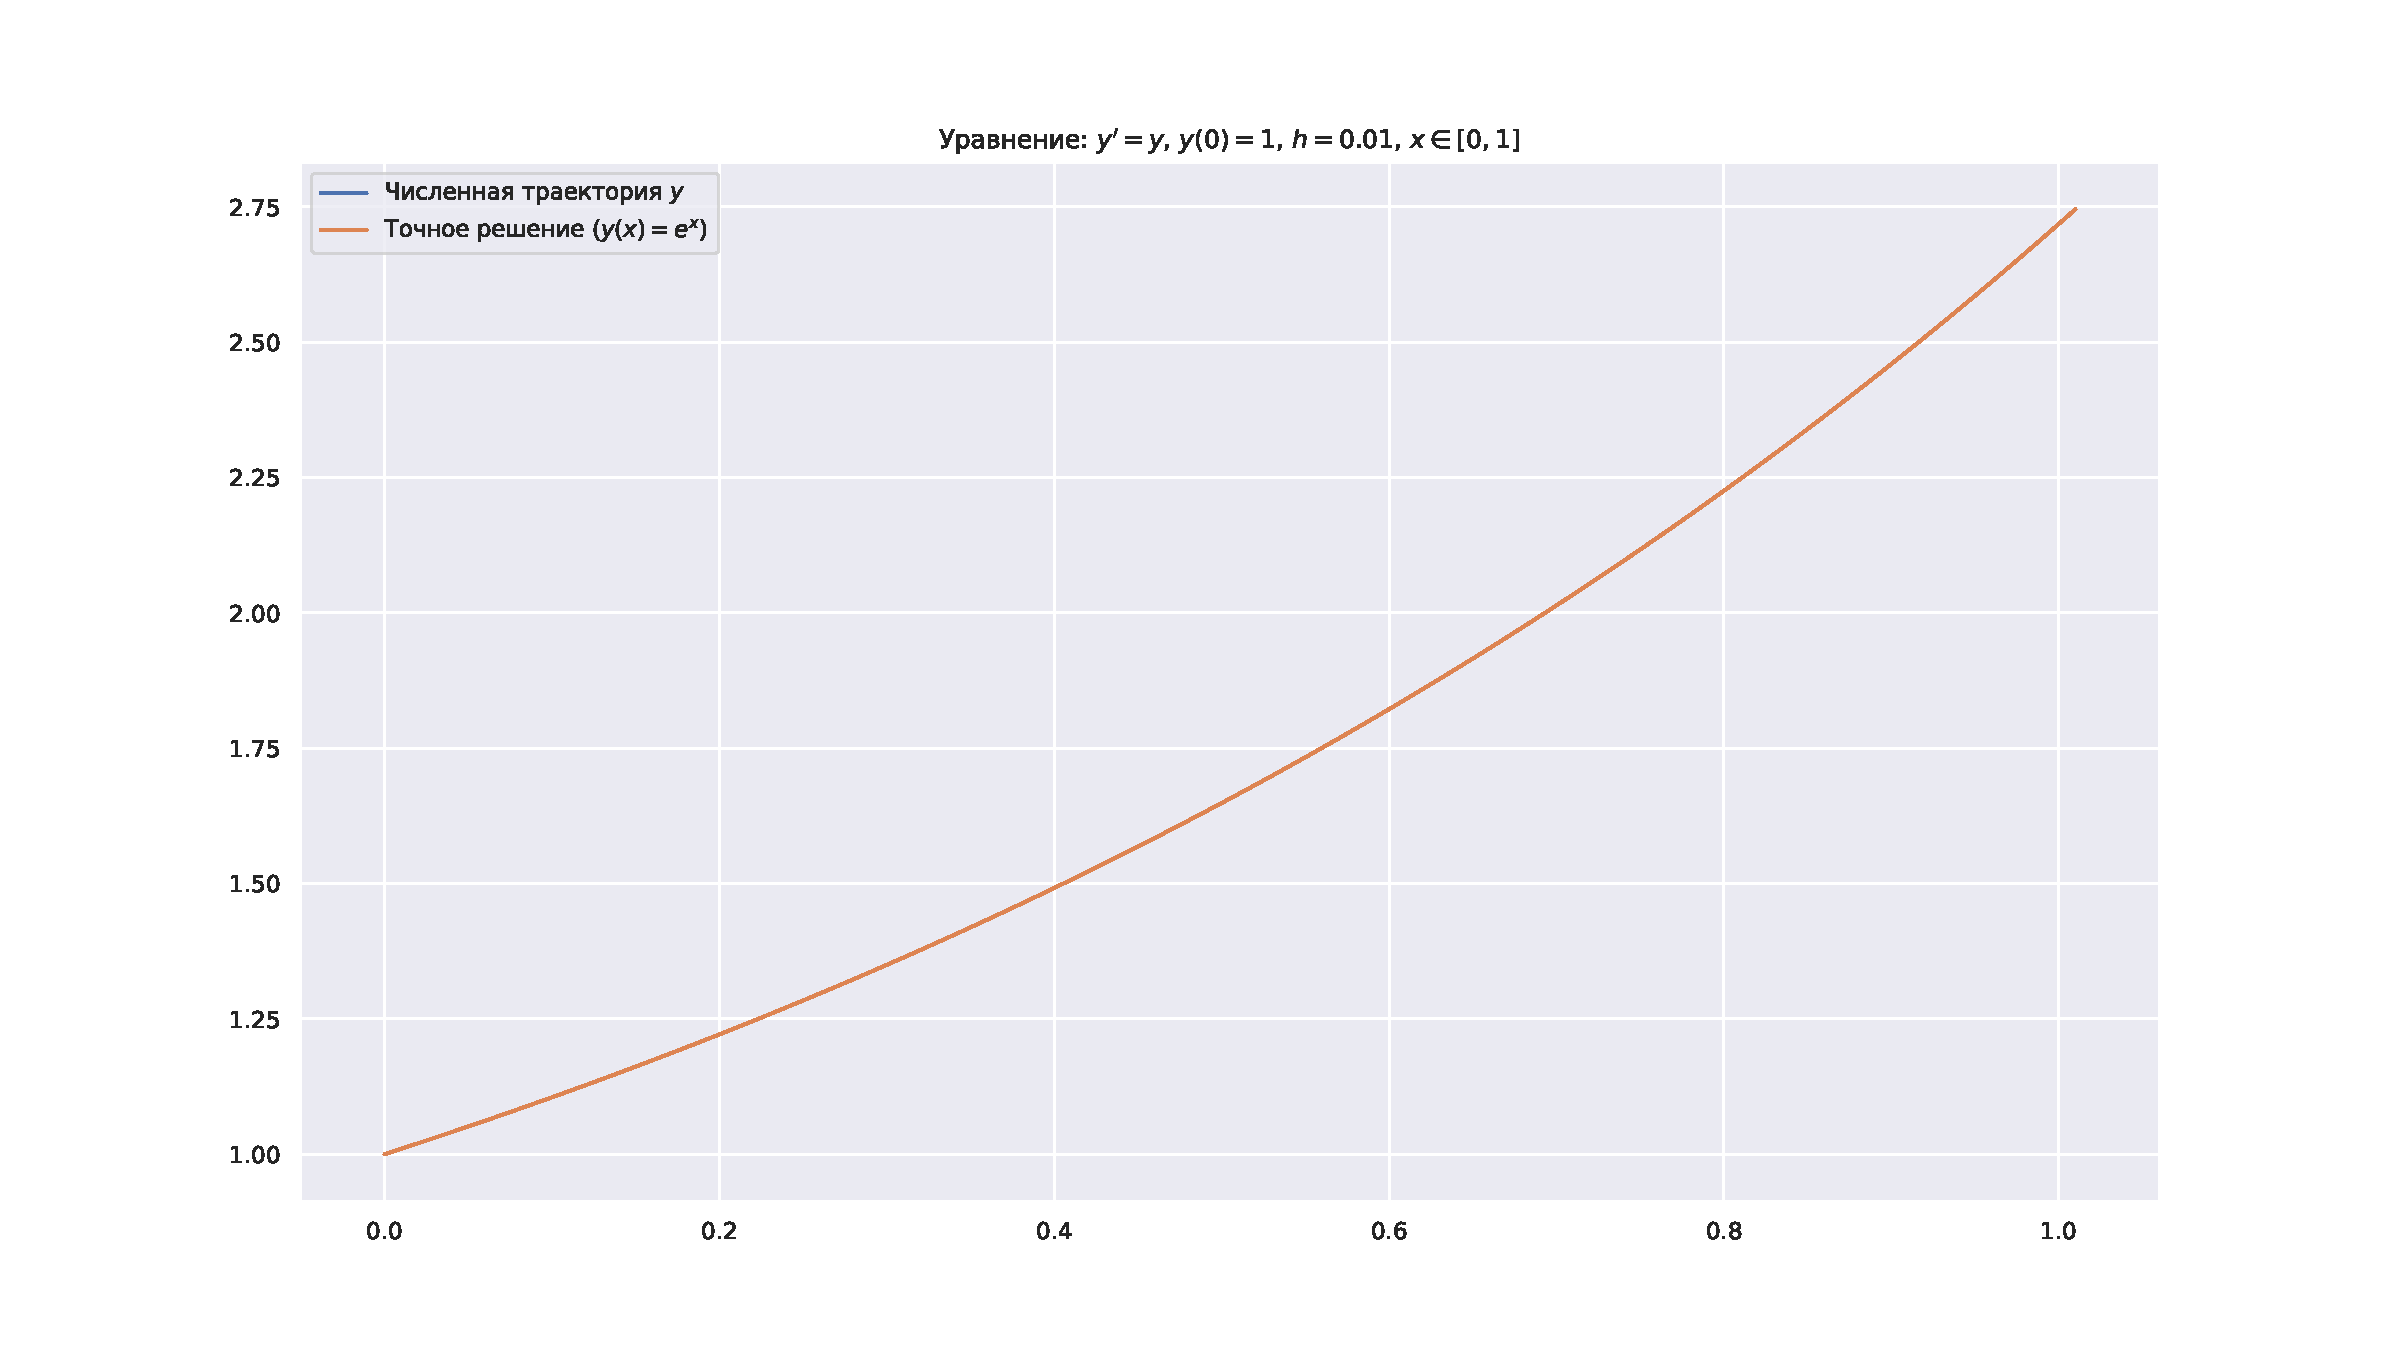
\includegraphics[scale=0.4]{figs/Test1.pdf}
    \caption{Результаты теста 1}
\end{figure}

\begin{figure}
    \centering
    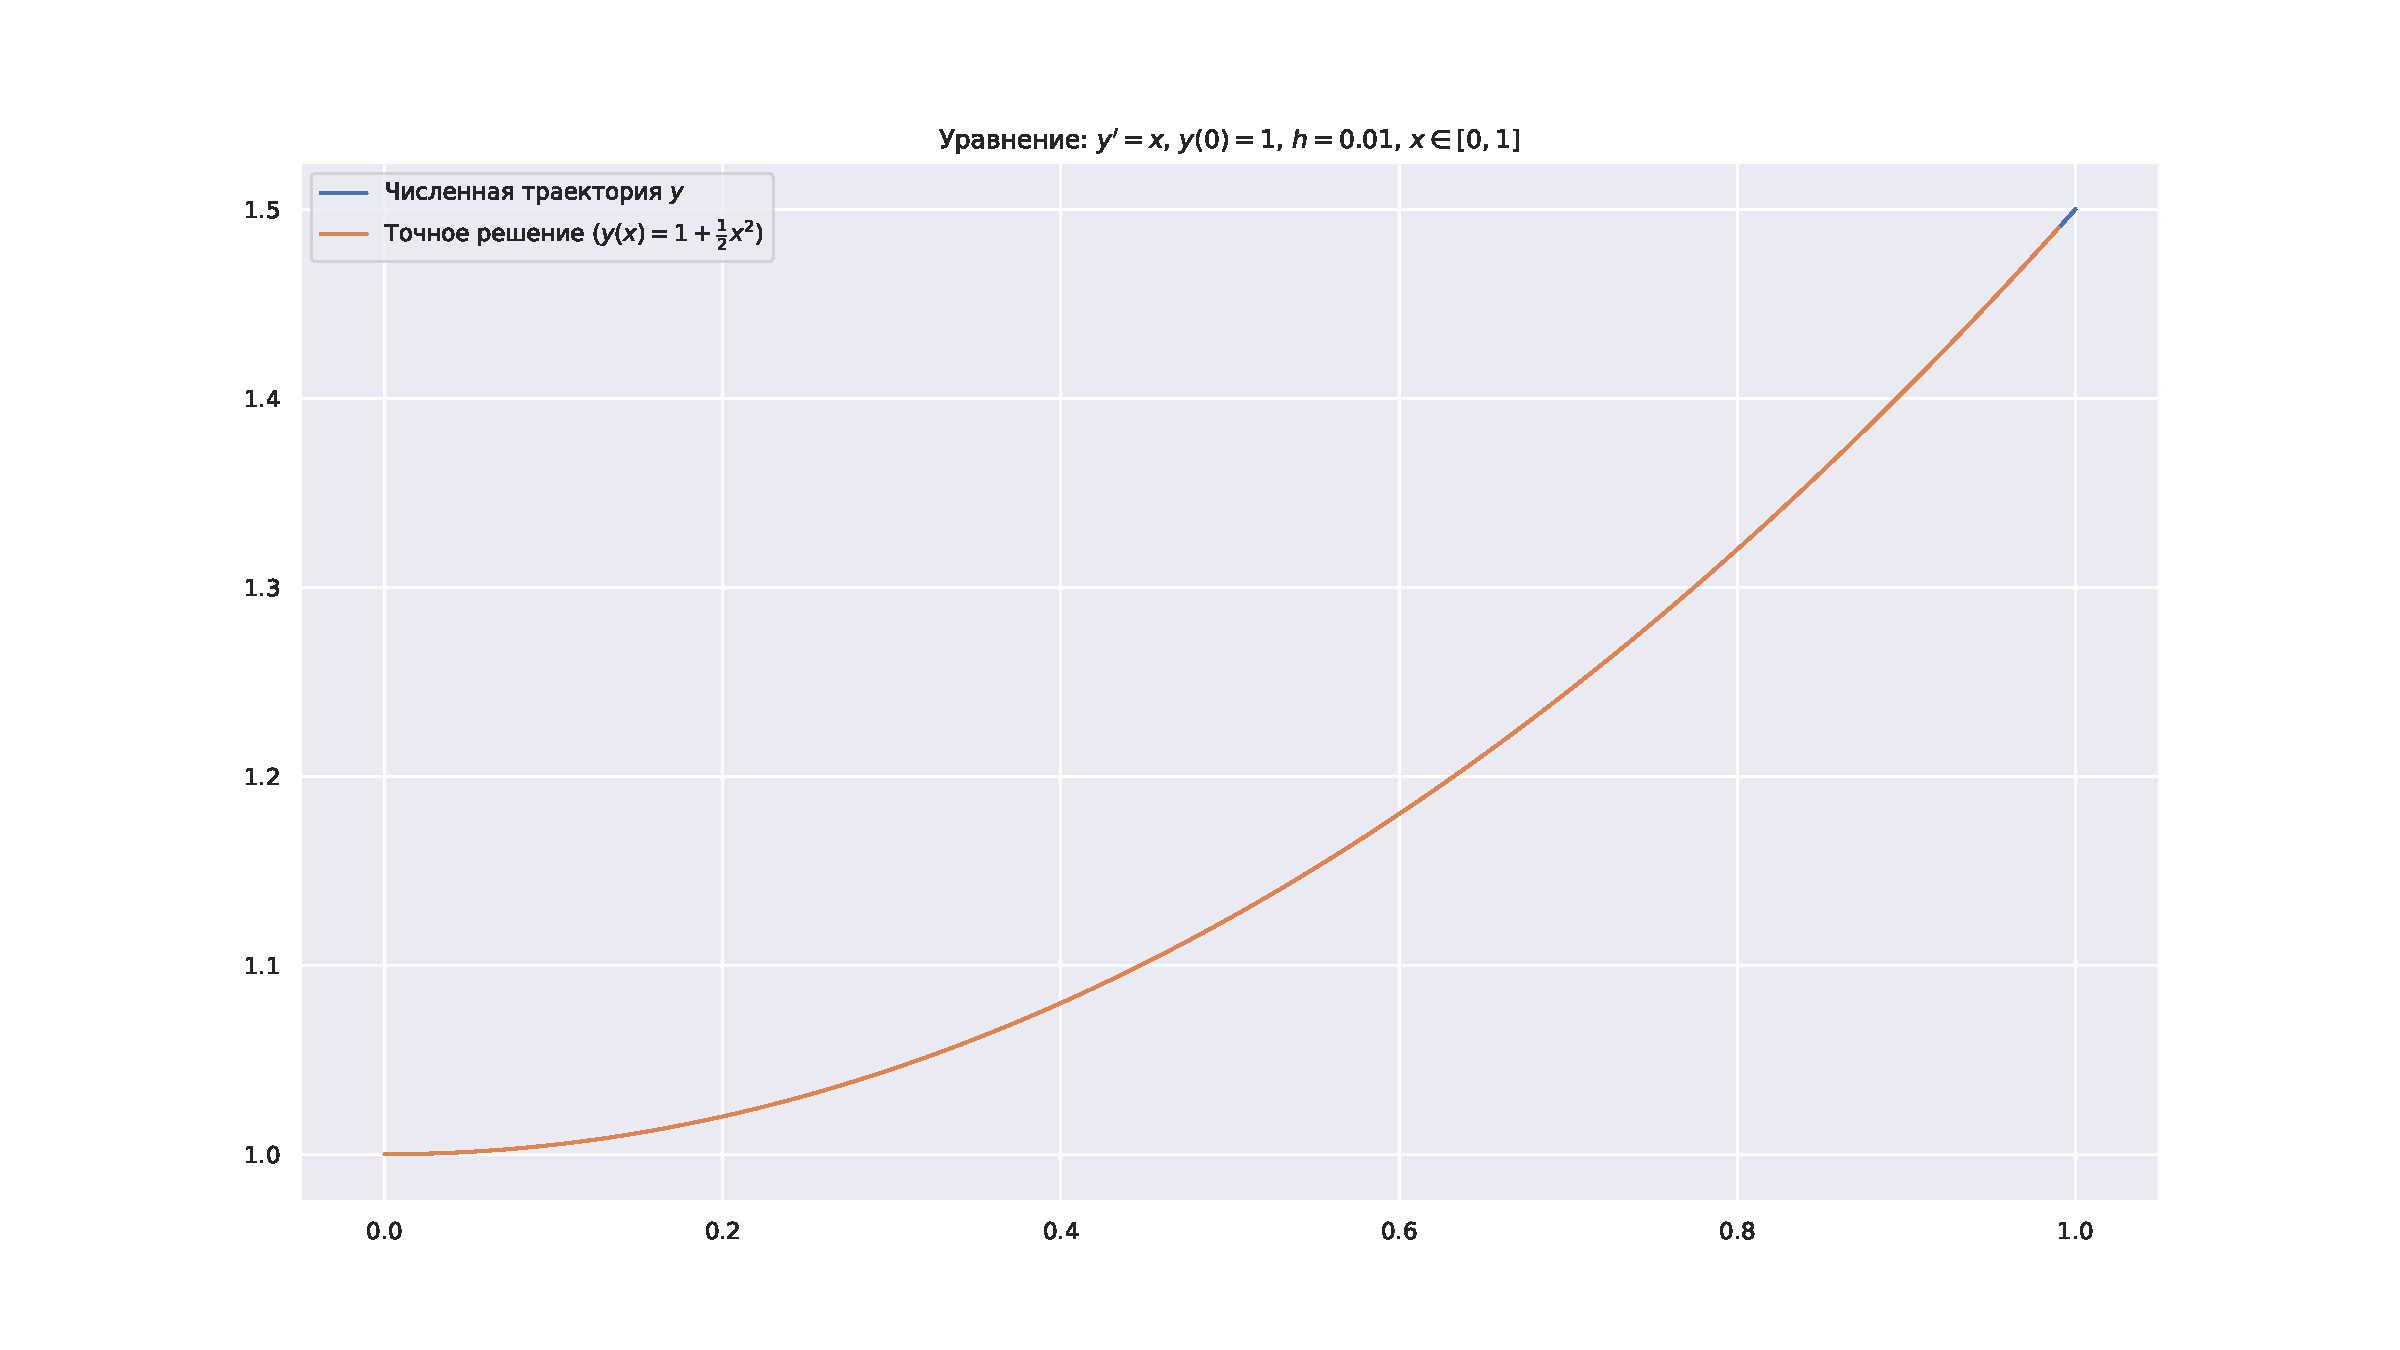
\includegraphics[scale=0.4]{figs/Test2.pdf}
    \caption{Результаты теста 2}
\end{figure}

\begin{figure}
    \centering
    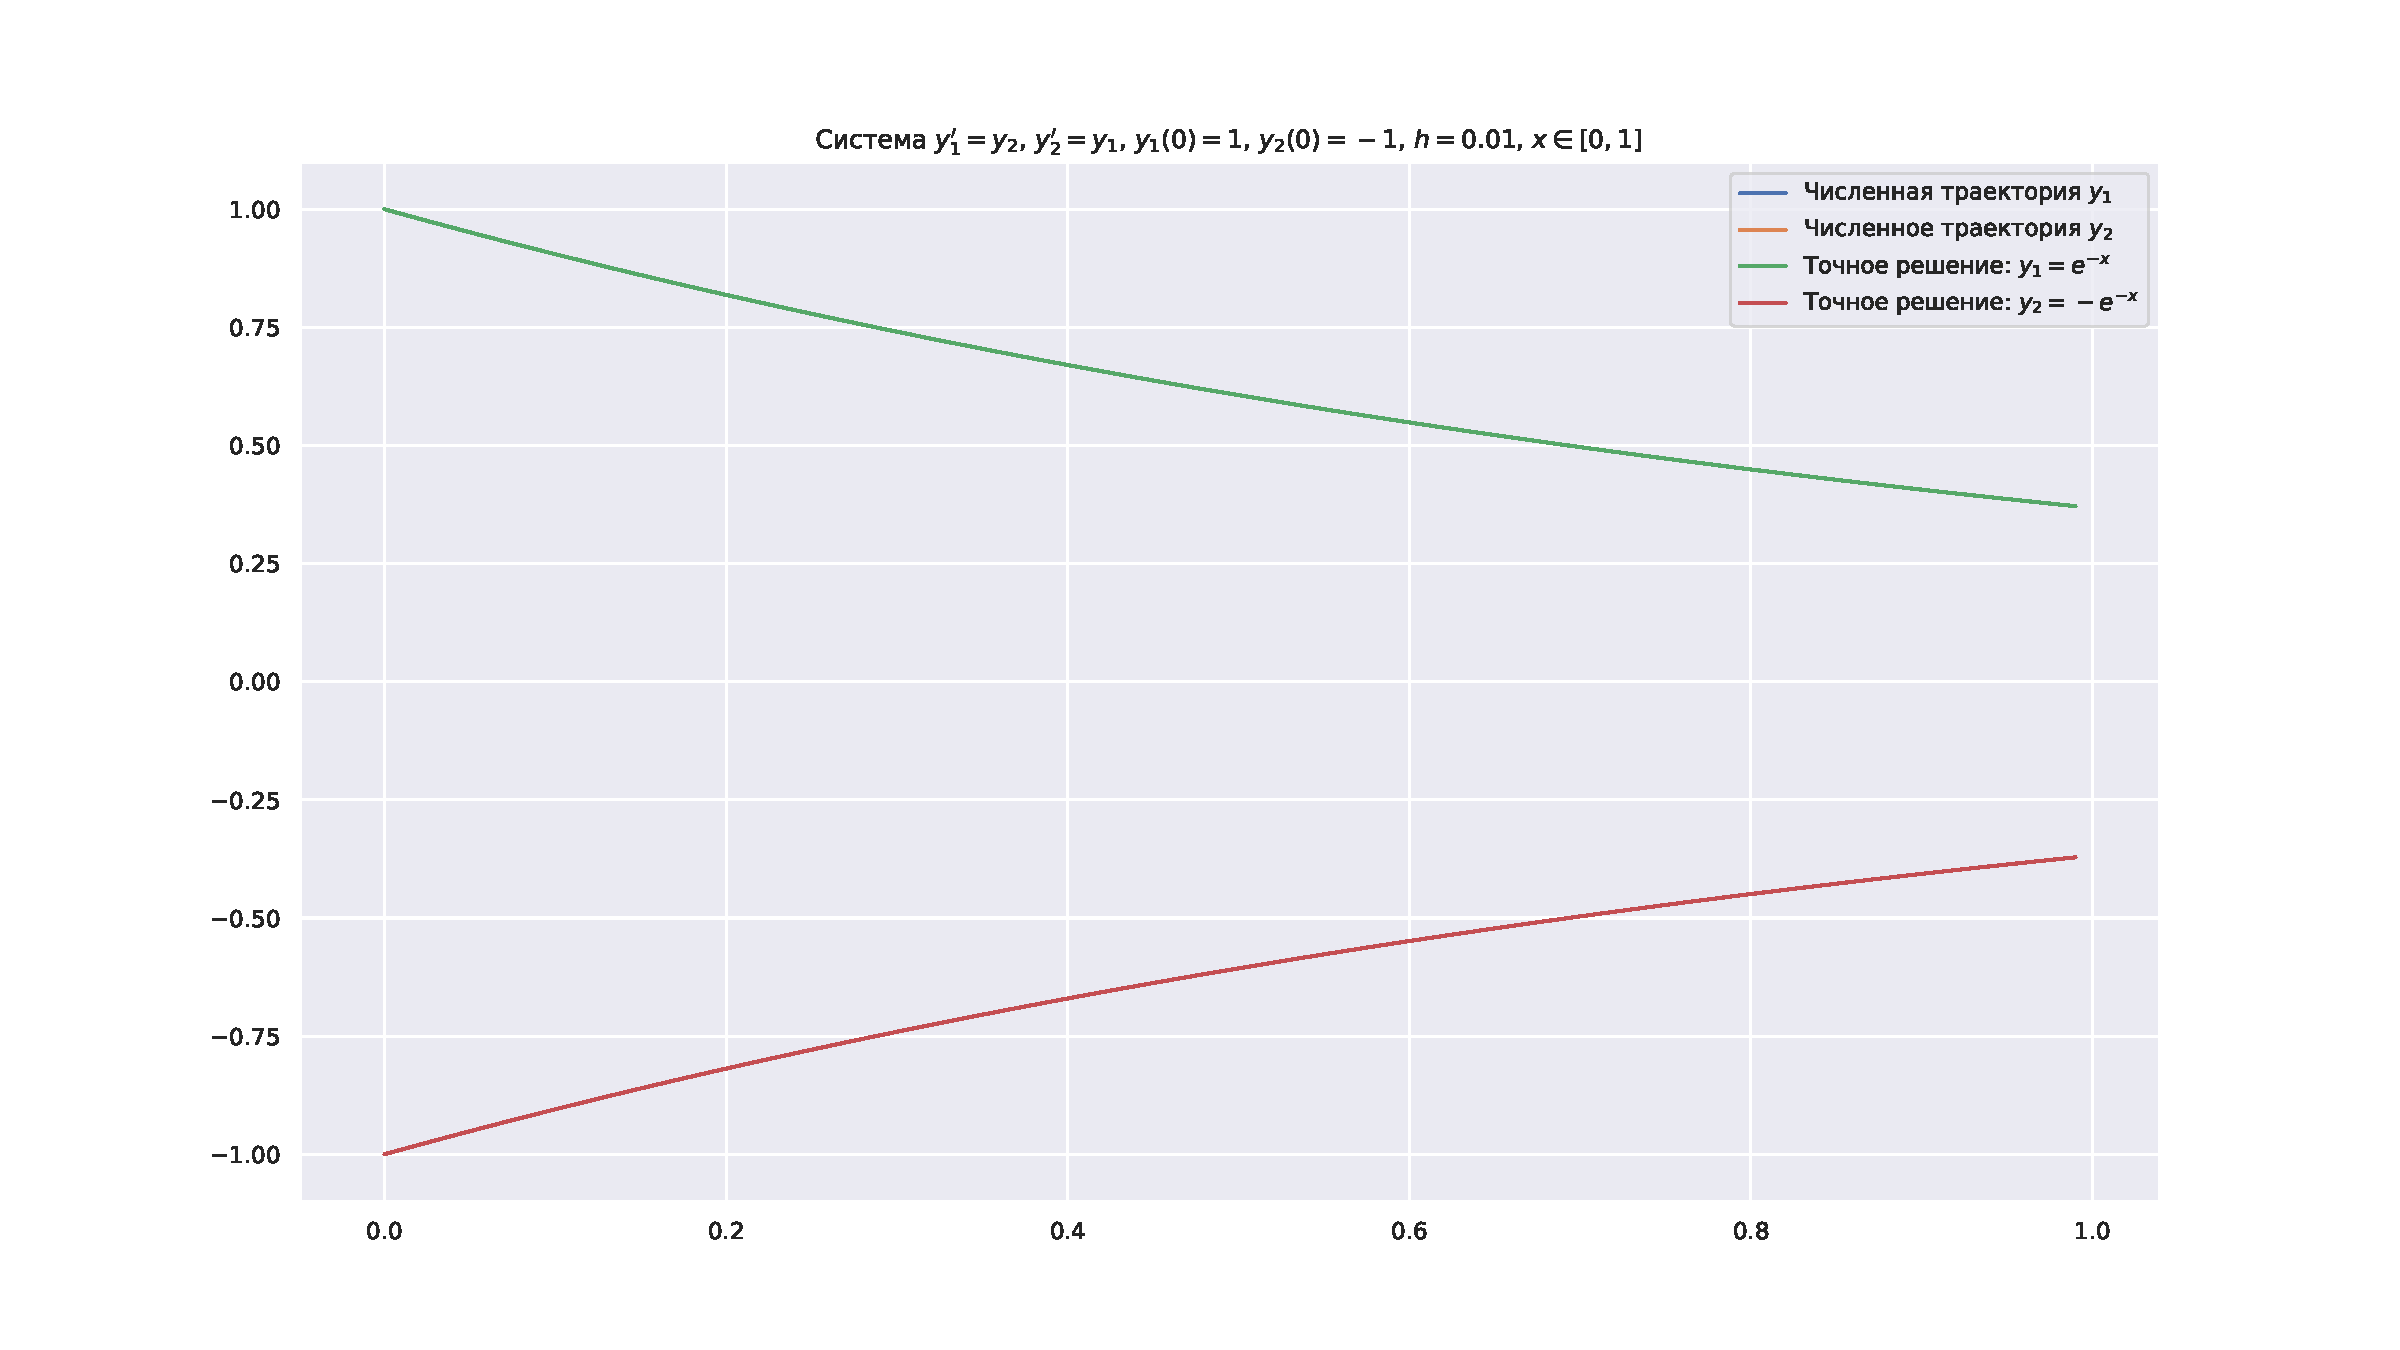
\includegraphics[scale=0.4]{figs/Test3.pdf}
    \caption{Результаты теста 3}
\end{figure}

\begin{figure}
    \centering
    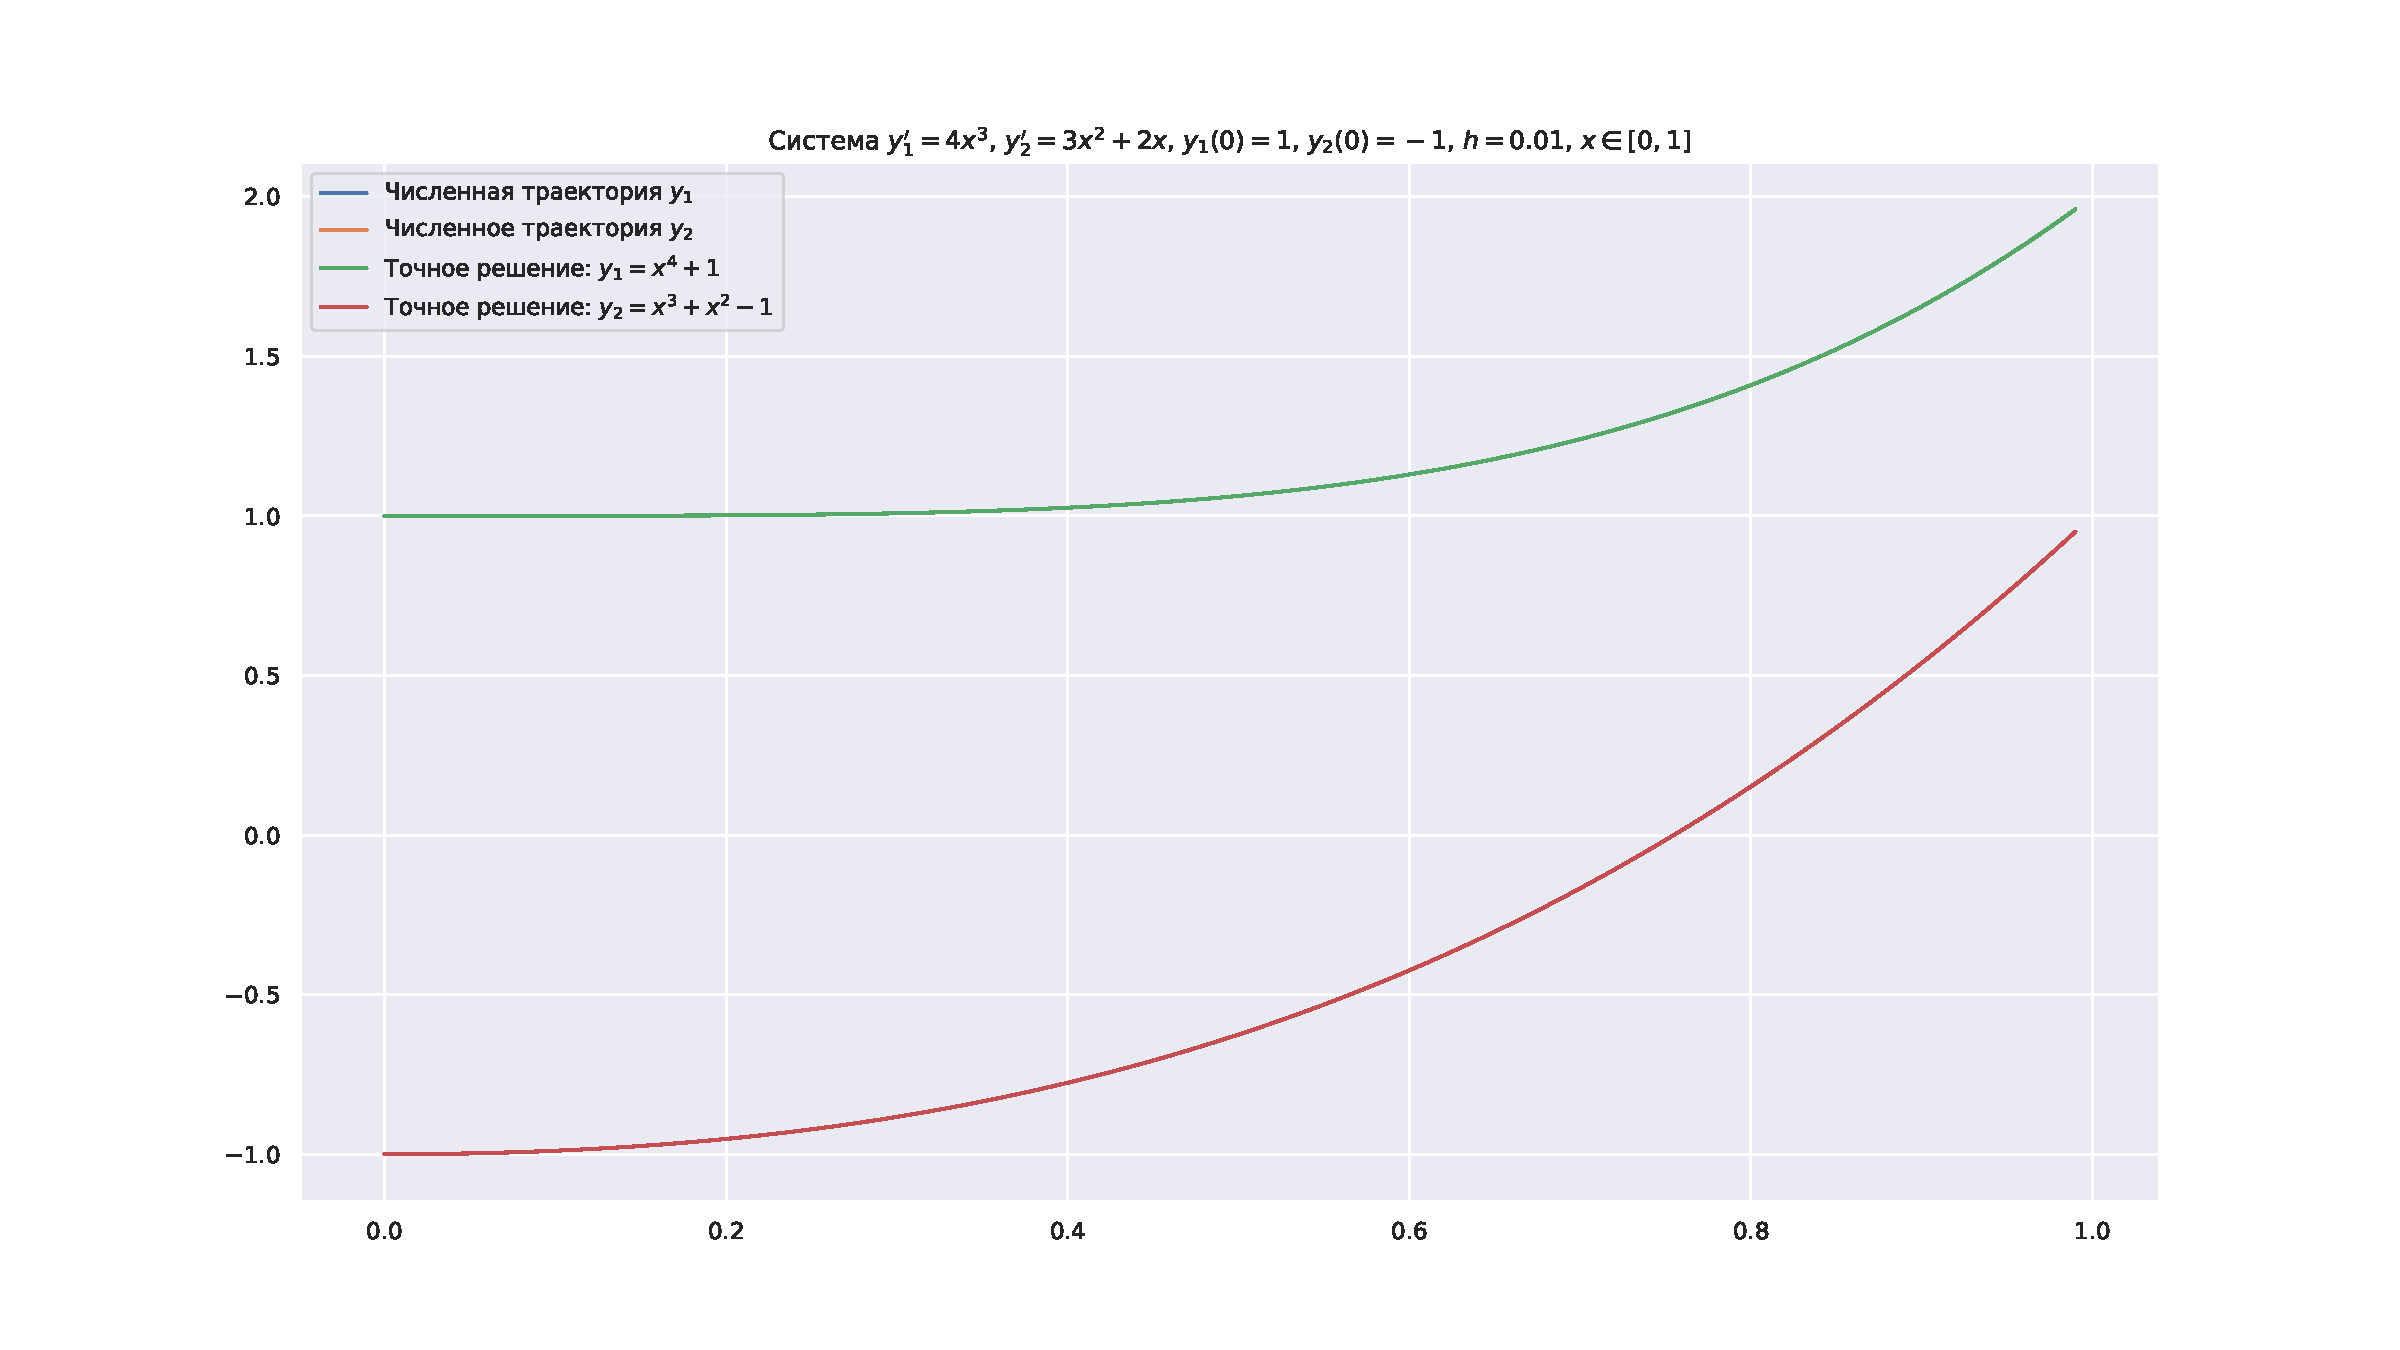
\includegraphics[scale=0.4]{figs/Test4.pdf}
    \caption{Результаты теста 4}
\end{figure}

\begin{figure}
    \centering
    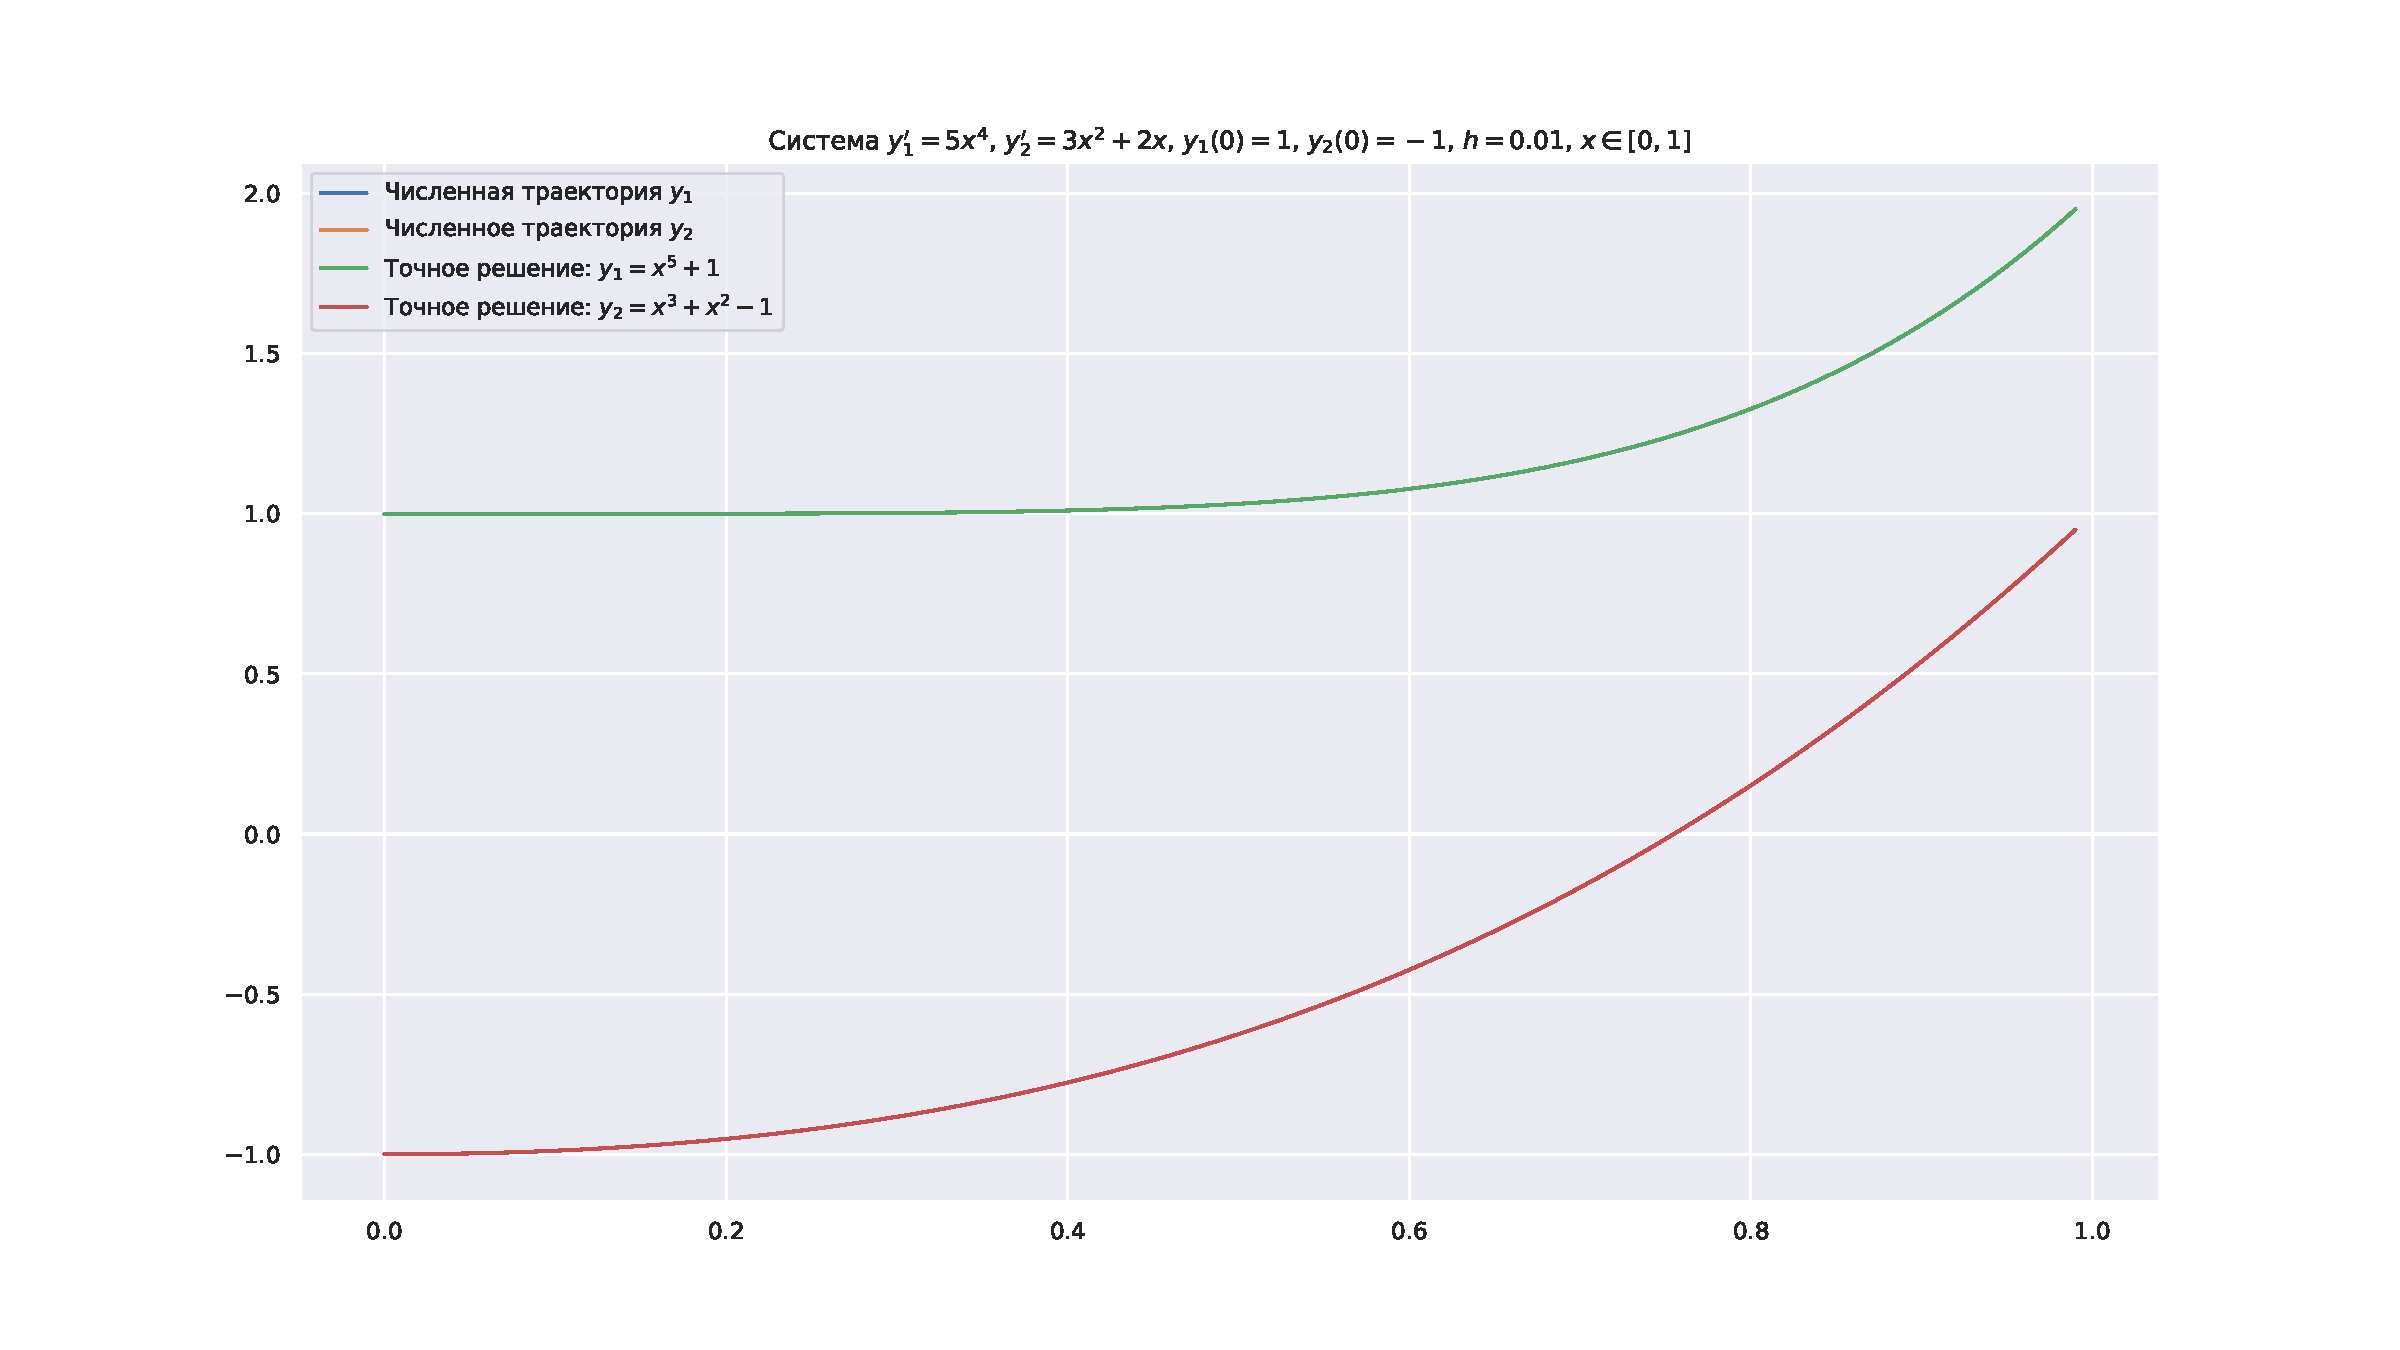
\includegraphics[scale=0.4]{figs/Test5.pdf}
    \caption{Результаты теста 5}
\end{figure}


\end{document}